\subsection{研究方法}
\subsubsection{数据组织与时间切分}
数据获取以1个新疆主研究场站、连续24个月历史记录为目标，连续12个月为启动场站方法验证的最低覆盖要求；不足24个月时据实缩小验证范围。核心字段包括交流侧功率、时间戳、装机容量和运行状态，地面辐照度、温度作为首批气象变量，NWP与卫星产品在取得授权且获取时间可追溯后逐项加入。第2场站仅用于扩展验证。时间统一为北京时间（UTC+8），同时保留原始时间、时区和数据实际获取时刻；太阳高度角由场站经纬度与对应时刻计算，避免地方太阳时与北京时间混用。将高频记录按15分钟窗口聚合，以窗口结束时刻标记时间，$p_t$对应$(t-15,t]$内的功率均值；气象变量同样取窗口内有效观测均值，运行状态保留异常标记；低于所需时间分辨率的数据不通过插值制造15分钟爬坡标签。以装机容量归一化功率，保留容量调整记录。训练前核验功率单位、时间重复、跳变、缺测、检修和限电标记；无运行状态证据的异常不直接标为天气事件。

对时刻$t$的预测，只使用获取时刻不晚于$t$的数据。NWP按起报时刻、预报有效时刻和实际获取时刻匹配，卫星产品按实际处理延迟入模。ERA5再分析仅用于离线天气描述或明确标注的理想输入对照。缺少可追溯NWP时，主任务使用历史观测与功率，不把未来实况填入预测端。气象状态用于模型选择时须在$t$可知；未来实况天气标签只用于事后分层评价。夜间及停限机时段分别报告：事后获知的停机可以从气象机制分析中剔除，但应保留在全运行时段的预报评价中并说明原因。

采用连续时间块组成训练、验证、初始校准和测试集合，按时间先后分配，分别占50\%、15\%、15\%和20\%，按完整日确定边界，四者用途互不替代。24个月数据可使训练段覆盖一个完整年周期，最终测试约覆盖4.8个月；各集合均列出实际月份，季节结论限定于测试段实际覆盖范围。仅有12个月记录时沿用同一比例开展方法验证，不作跨年泛化结论。多时距样本仅在目标窗口完全落入所属集合时使用，集合边界隔离4小时；模型超参数和告警阈值在验证阶段确定，测试前锁定。测试段按自然月连续回放，每15分钟发布一次预测；如取得第2场站授权，另作跨站检验，单站结果不外推为所有新疆基地。归一化、插补参数、变量选择与小波尺度均只依赖训练信息；测试期间仅按预先确定的规则更新校准，模型选择不再使用测试效果。

\subsubsection{天气状态与评价块划分}
发布时刻的天气分组以辐照状态为代理。取$(t-60,t]$内四个完整15分钟区间的水平面总辐照度均值，以固定Haurwitz晴空模型在同一窗口的均值作参照，得到四个辐照指数；晴空参照仅由场站位置、时间及固定标准大气参数计算，按1分钟网格求均值。四项观测须质量合格且已到达，窗口内各分钟太阳高度均不低于10度。记指数中位数为$m_t$、相邻指数绝对差的最大值为$v_t$，阈值采用训练段$m$的75\%分位数及$v$的25\%、75\%分位数，经验分位数取排序后第$\lceil np\rceil$项，进入验证前冻结。$v_t>Q_{0.75}(v)$记为快速变化；否则，$m_t\geq Q_{0.75}(m)$且$v_t\leq Q_{0.25}(v)$记为高指数平稳；其余有效样本记为其他状态。缺测、迟报、低太阳高度或仅有组件平面辐照时记未知，回退总体模板；指数超过1不直接判为异常。这些类别描述相对辐照水平与变化，不直接等同于晴天、云团或沙尘。
% Haurwitz输入与GHI输出依据：https://pvlib-python.readthedocs.io/en/stable/reference/generated/pvlib.clearsky.haurwitz.html

沙尘另按可核验天气记录分为发生、未发生与未知，记录来源及有效时段在测试前确定；用于发布时诊断的记录须已取得且覆盖$t$，事后补齐记录仅作事后分析。天气条件模板只按上述辐照类别匹配，不再交叉细分沙尘类别；报告各类模板数量与回退比例。若缺少水平面辐照而全部回退总体模板，则天气条件选择的增益记为未能检验。

样本量按北京时间自然日组成评价块，同日重叠窗口及多次事件不重复增加块数。仅在天气记录明确属于同一跨日过程，或同一实测事件段跨越午夜时，合并所涉相邻日块；保留合并依据，不仅因类别相同而合并。各方法共享块划分，缺测不视为无事件，也不跨缺测空档合并事件。该划分用于过程计数，不预设各块统计独立，跨块依赖在分块重采样中处理。

\subsubsection{多尺度分位数建模}
以过去24小时、共96个采样点作为输入窗口，在窗口内进行小波分解，形成慢变与快变分量，任何边界处理均只使用$t$及以前的观测；不对包含测试未来值的全序列一次性分解。主模型在申请人已有DWT-Former多尺度结构上设置分位数输出，WaveKAN仅用于结构替换对照，复用已有研究代码与建模经验。引入气象外生变量时比较固定融合与天气条件融合，保持可比的参数规模、训练轮数和输入长度。主要模型与消融均采用3个随机种子重复训练，各次训练在单张现有GPU上完成，利用多卡并行运行独立实验。

设$p_{t+h}$为归一化实际功率，$\widehat q_{t,h}(\tau)$为$t$时刻对$t+h$的$\tau$分位预测，采用分位数损失
\[
\ell_\tau(y,q)=\bigl(\tau-\mathbf{1}\{y<q\}\bigr)(y-q).
\]
分位数网格采用0.05--0.95、间隔0.05的19个分位水平，两端以已知物理界限作有界延伸，尾部估计另作敏感性分析。输出分位数采用递增重排处理交叉，并将功率限制在当时已知容量对应的物理范围内。该处理并不证明预测分布正确，其效果仍需在独立时段检验。模型与持续性、晴空归一化持续性、线性预测、分位数梯度提升及标准Transformer比较；点预测基线用于误差比较，概率评分比较限于提供分位数或事件概率的模型，以保证评价对象一致。

\subsubsection{滚动校准与可靠性评价}
以目标覆盖率$1-\alpha$的原始区间为起点，对已获真实值的历史样本计算非一致性分数
\[
s_{i,h}=\max\{\widehat q_{i,h}(\alpha/2)-p_{i+h},\ p_{i+h}-\widehat q_{i,h}(1-\alpha/2)\}.
\]
在$t$时刻，只从满足$i+h\leq t$且真实值已经到达的样本中选取校准分数；缺测或迟报样本等待到齐后再用。用预定窗口的分位数修正区间端点，校准量取非负值以避免区间反转，再按固定规则约束到物理范围内，所有评分均评价处理后的最终区间。有限校准样本的分位位置采用共形化分位数回归的相应修正\cite{romano2019cqr}；逐时距更新，比较不校准、静态校准和滚动校准。以80\%和90\%预测区间为主要报告层级，滚动校准采用最近30天的已到达标签，每15分钟更新；14天与60天窗口用于敏感性分析。静态校准使用初始校准段末30天的有效样本，测试期间保持校准量不变；30天滚动校准从同一批样本起步。14天与60天窗口分别用初始校准段末对应时长初始化，覆盖不足时仅使用该段已到齐样本，报告实际天数，随后随标签到达补足窗口。对时间相关和分布漂移条件，报告经验覆盖与区间评分，不承诺任意漂移下的有限样本覆盖保证。

逐时距计算平均分位数损失、覆盖偏差、归一化区间宽度和区间评分，并按天气与季节给出样本量。点预测另报归一化平均绝对误差（MAE）与均方根误差（RMSE），避免夜间零值使全日指标显得过好。分层样本不足时保留总体校准并单列该组不确定性，不事后调节分组直到指标合格。比较以同一测试时间块的配对差异为主，不把单个时间点当独立重复。

\subsubsection{同边际轨迹与爬坡定义}
设$\mathcal I_t$为$t$时刻可用信息，$\delta$为固定爬坡间隔，定义
\[
R_{t,h,\delta}=p_{t+h+\delta}-p_{t+h},\qquad
E^+_{t,h}=\mathbf{1}\{R_{t,h,\delta}>r\},\quad
E^-_{t,h}=\mathbf{1}\{R_{t,h,\delta}<-r\}.
\]
这里只评价两个端点之间的净变化，$h>0$且两个端点均落在预测采样网格上，$h+\delta$不超过最大预测跨度；不把它等同于窗口内最大瞬时变化。主事件定义为30分钟功率净变化幅度超过装机容量的20\%，即$\delta=30$分钟、$r=0.20$，10\%与30\%阈值用于敏感性分析。主要概率终点为发布时间后第60至90分钟的下降爬坡，即$p_{t+90}-p_{t+60}<-0.20$；其他时距和上升事件为次要或探索性检验。上述阈值为本研究统一采用的分析判据。完成数据核验后、查看留出测试标签前，将主事件、告警选择规则、天气分组、模板回退和事件匹配参数保存为统一版本；业务方反馈另行记录，不据此回改主检验定义。上下坡分别评价；跨夜间、缺测或停限机的标签按既定规则分层，防止把日出日落和非气象停机误解释为天气扰动。

轨迹构造采用已学习的单调分位数网格；两级区间校准是额外可靠性诊断，不能被视为整条累积分布已校准。对每个时距的同一预测分位数网格抽取同一组$M$个样本，保留依赖组根据历史完整误差向量的跨时距秩关系逐列排序，独立组则对各列独立置换。两组每一列的样本数值完全相同，只有行内时间配对改变，以隔离时间依赖贡献。历史模板借鉴Schaake shuffle的经验秩思想\cite{clark2004schaake,schefzik2013ecc}，所用残差来自历史滚动留出预测，不能采用模型在自身训练样本上的拟合残差。验证开始前，模板由训练段内部的滚动留出预测初始化；验证、初始校准和测试按时间先后回放，仅追加当时已经到齐的完整残差，避免后续数据参与告警阈值选择。仅使用整条预测轨迹真实值均已到达的样本，将当前$t$时可知天气与各历史预测发布时已知的天气状态匹配，不按历史事后天气筛选模板；同类天气模板不足100条时回退总体模板。设置总体历史秩、发布时刻天气条件历史秩与独立随机排序三个对照，独立排序重复5个随机种子。每次生成100条轨迹，并以50条、200条检验抽样敏感性；所选模板池不足所需条数时，按完整误差向量有放回抽样，重复样本的并列秩使用固定随机种子打破，并报告独立历史样本量。若总体历史依赖有效而天气条件选择无效，只接受前一层结论。根据第$m$条轨迹计算事件，得到
\[
\widehat\pi^+_{t,h}=\frac{1}{M}\sum_{m=1}^{M}
\mathbf{1}\{p^{(m)}_{t+h+\delta}-p^{(m)}_{t+h}>r\},
\]
下降概率同理。边际区间校准不自动保证联合事件概率校准，因此事件概率另用Brier评分、相对训练期天气/时段事件率基线的技能分数、可靠性图和事件样本量检验；路径关系辅以变差函数评分\cite{scheuerer2015variogram}。直接增量分位数或分类模型作为更简单的补充对照，并明确其没有“同边际”这一受控条件。

\subsubsection{预警评价与统计分析}
概率评分使用未经告警阈值化的全部有效概率。告警阈值在验证集以0.05为步长搜索0.05--0.95，同时满足每个有效日平均误报事件不超过1次、误报告警时间比例不超过5\%时，选择事件召回率最高的阈值；并列取较高阈值，无可行阈值或无该类实测事件时不发出该类告警，仍保留概率评分。两个上限为研究预设约束，不代表业务标准或测试期保证。测试期锁定阈值，报告实际误报次数、时间比例、精确率、召回率和提前量。

告警主评价采用正常并网且两个目标功率区间内太阳高度均不低于10度的日照窗口；停限机及全运行评价另报。概率与告警的配对比较均取各参评方法预测齐全、真实标签合格的共同窗口，另报因缺报共同剔除的窗口比例与事件数。按15分钟发布时间网格，每个有效窗口计15分钟评价时间，告警且对应实测窗口不满足事件判据时计15分钟误报时间；二者相除得到时间比例。该指标衡量发布网格上的告警负担，不等同于物理爬坡持续时长。有效日数为逐日有效窗口数占该日太阳几何应有窗口数的比例之和，几何窗口数为零的日期不计，各方法使用同一分母。

分别将已触发告警的预测窗口和满足判据的实测窗口按相邻重叠关系合并为事件段，不跨缺测空档合并，起点取最早窗口起点。以起点相差不超过15分钟为容差进行一对一匹配，告警须在实际事件起点前发布，每起事件仅计一次命中，提前量取首次有效告警至实测起点的间隔。事件匹配允许起点容差，时间误报则按窗口标签严格计数；长告警段即使命中一次，其延续到非事件窗口的部分仍计误报时间。事件与窗口指标同时报告，并给出精确率--召回率（PR）曲线及无技巧参考。无告警、无事件或无有效窗口造成分母为零时，相应指标记为不适用并报告计数。

以各方法共同的评价块进行配对分块自助，多日跨度根据训练期误差自相关选定；将合并后的评价块视为不可分单元，有放回抽取相邻块组成达到预定跨度的区段，在完整块边界停止，并按抽得的全部有效窗口计算平均差值。重复2000次，报告95\%置信区间及块长敏感性结果。主要检验为总体历史秩组减独立组的Brier差值$D_0$，天气条件历史秩组减总体历史秩组的$D_1$为预设次要检验，测试后不交换顺序；差值区间完全低于零才支持改善，跨零记为证据不足。多时距、多天气结果完整报告，探索性比较单列。每一重点分层至少积累30个含该类状态或事件的有效日/过程块后再作定量判断；事件结论要求至少30个含相应事件的块，不能以无事件日补足。未达门槛时仅报个例、样本量与描述性结果；达到门槛后仍结合效应与区间宽度评价证据，不视为独立性或统计功效保证。

\subsection{技术路线}
\subsubsection{总体路线}
以获得合法使用条件的功率和气象数据为起点，先建立发布时刻的信息集合并识别可利用的时间尺度，内容一据此输出可追溯样本和变量选择依据。内容二在同一数据划分上训练概率模型并保存边际预测、到齐标签和连续误差向量；内容三接收这些产物，通过同边际轨迹对照检验爬坡概率，再将验证集确定的决策规则接入离线原型。三项内容在数据、概率输出和事件评价之间依次衔接，最终以独立时间段与天气过程检验总体目标。
% NSFC-ILLUSTRATED BEGIN F02
如图~\ref{fig:xj-f02} 所示，总体研究框架：原始分位网格与完整历史误差进入爬坡分析，校准区间用于并行诊断。
\begin{figure}[htbp]
\centering
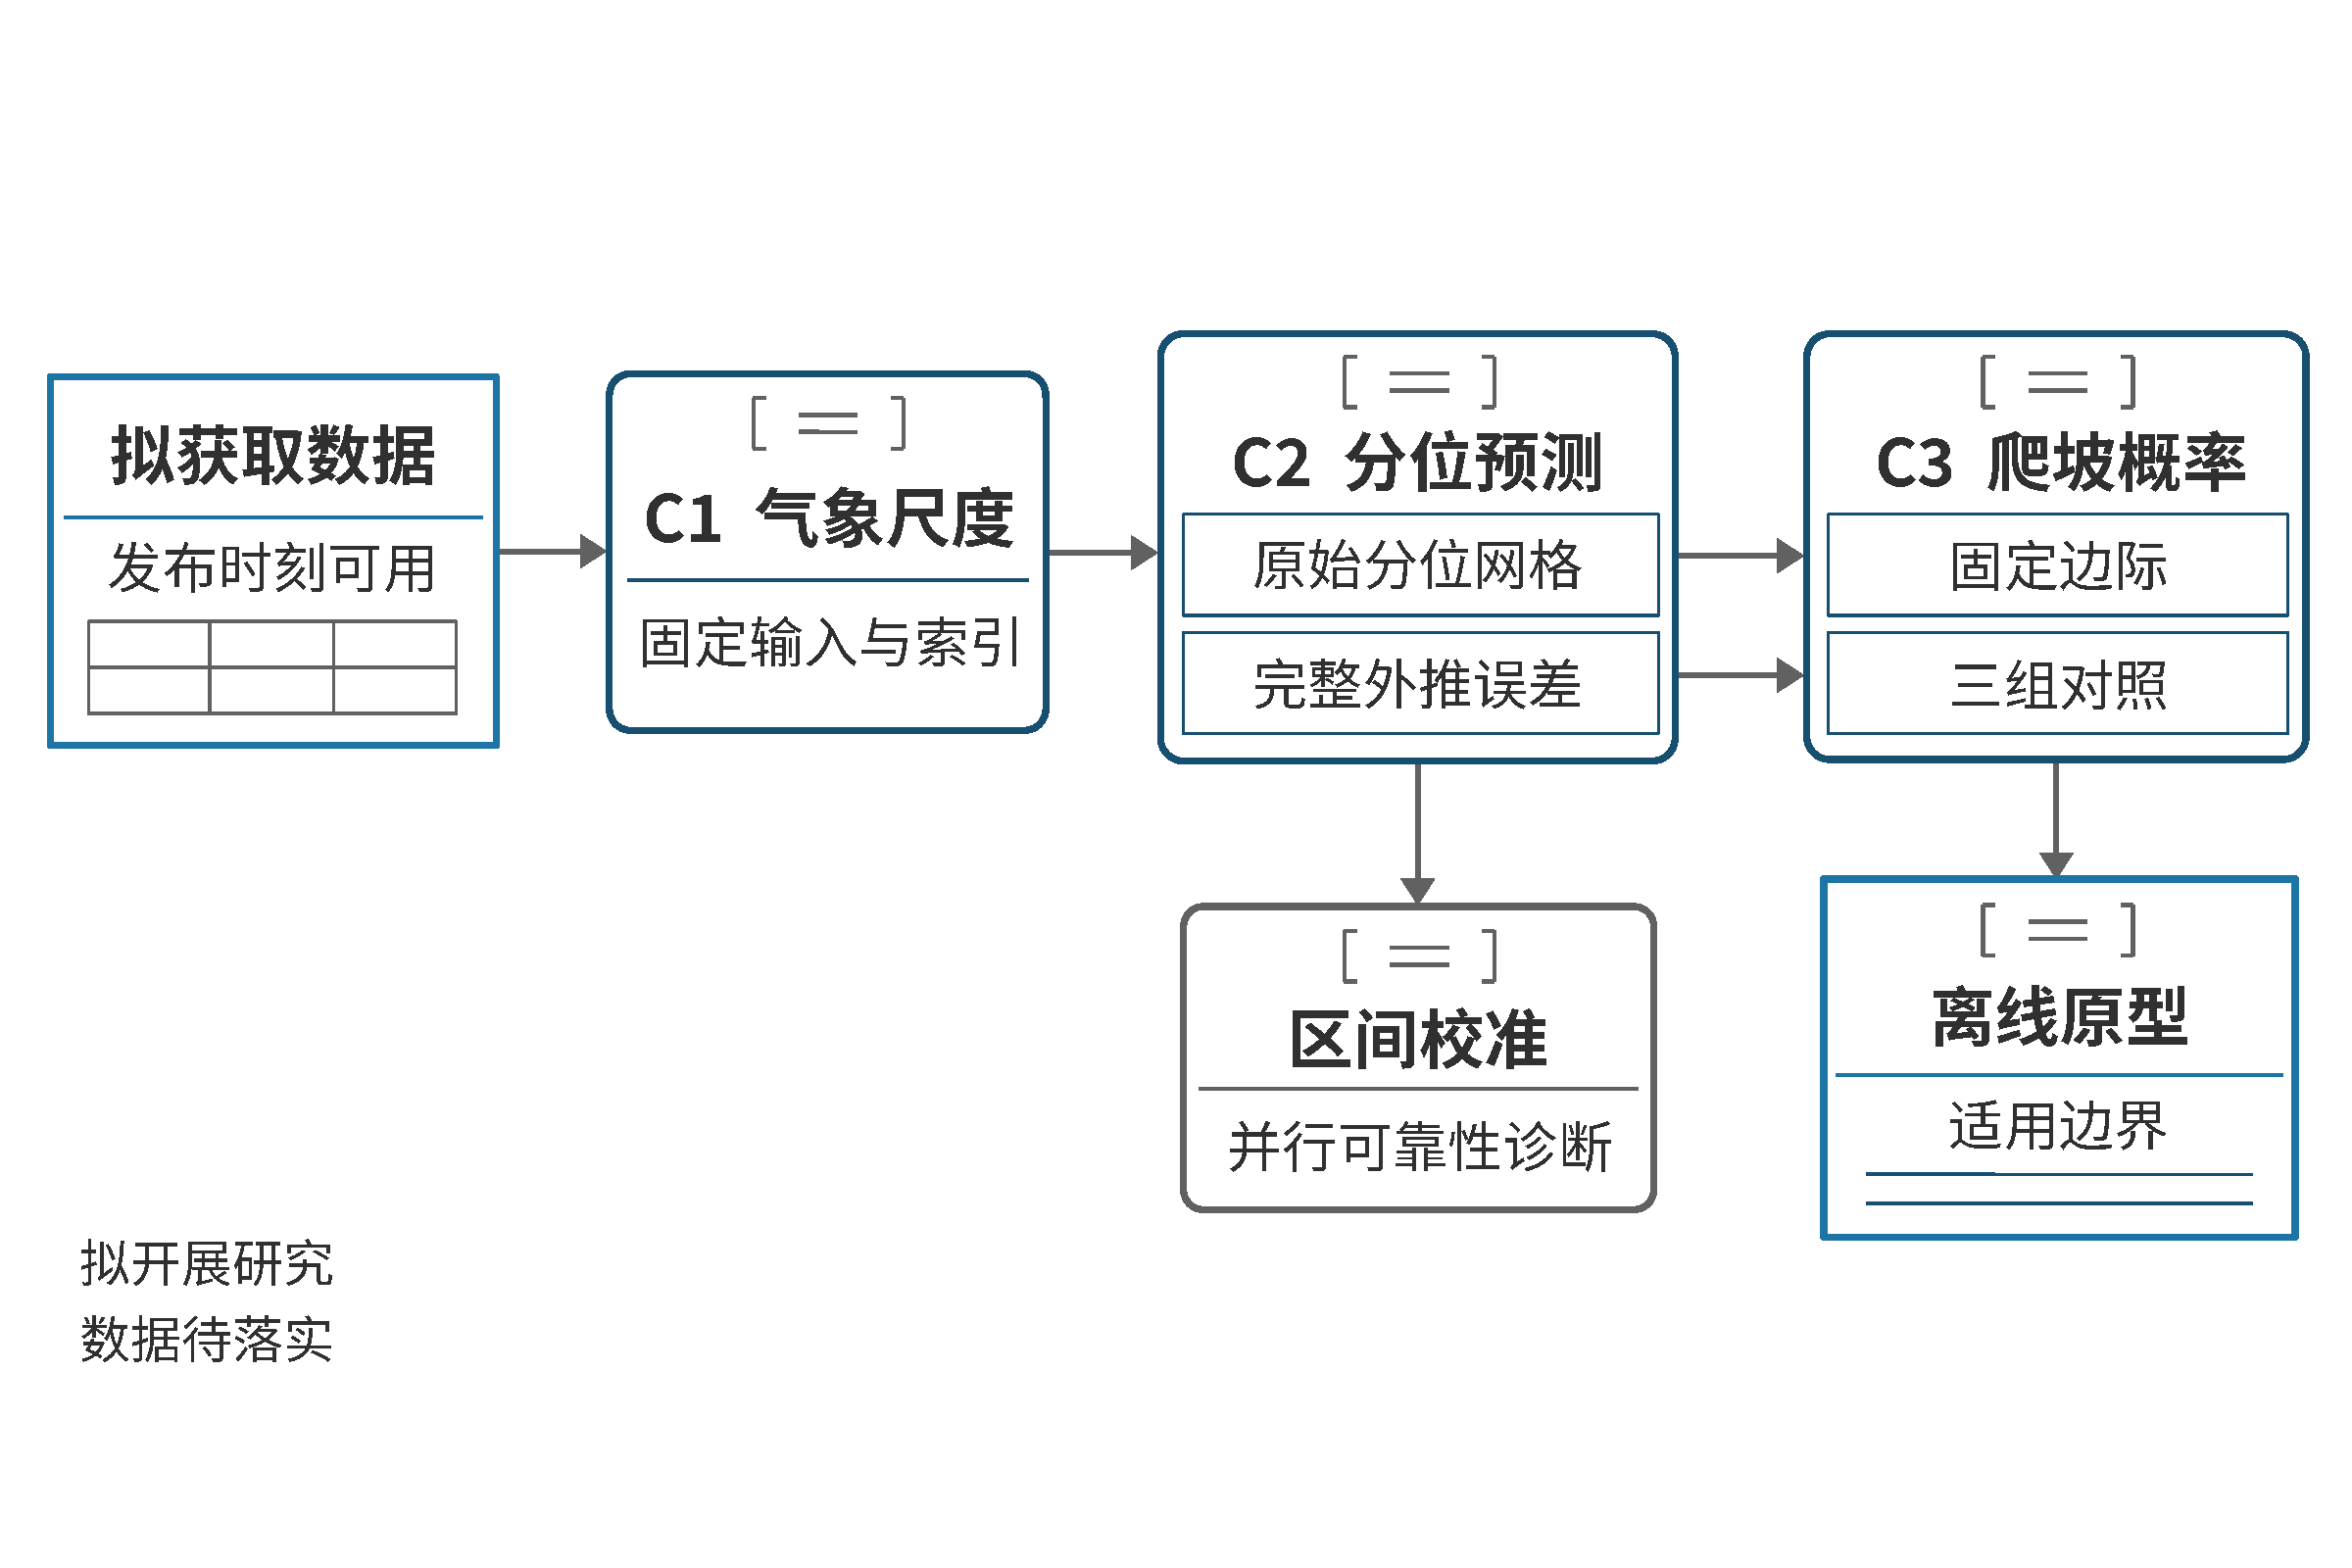
\includegraphics[width=0.94\linewidth]{figures/F02.pdf}
\caption{总体研究框架：原始分位网格与完整历史误差进入爬坡分析，校准区间用于并行诊断}
\label{fig:xj-f02}
\end{figure}
% NSFC-ILLUSTRATED END F02

\subsubsection{对应研究内容一的路线}
输入原始功率、气象与运行日志，完成授权核验、时间对齐和异常分层；以因果窗口提取尺度特征，在统一预算下进行逐源增量与变量消融。输出可复现数据清单、训练测试索引和尺度增益分析，用跨时间块的损失差异检验其稳定性。这些索引和保留变量成为内容二的固定输入。
% NSFC-ILLUSTRATED BEGIN F03
如图~\ref{fig:xj-f03} 所示，可用信息与跨尺度增益路线（数据按授权加入，变量选择不使用测试效果）。
\begin{figure}[htbp]
\centering
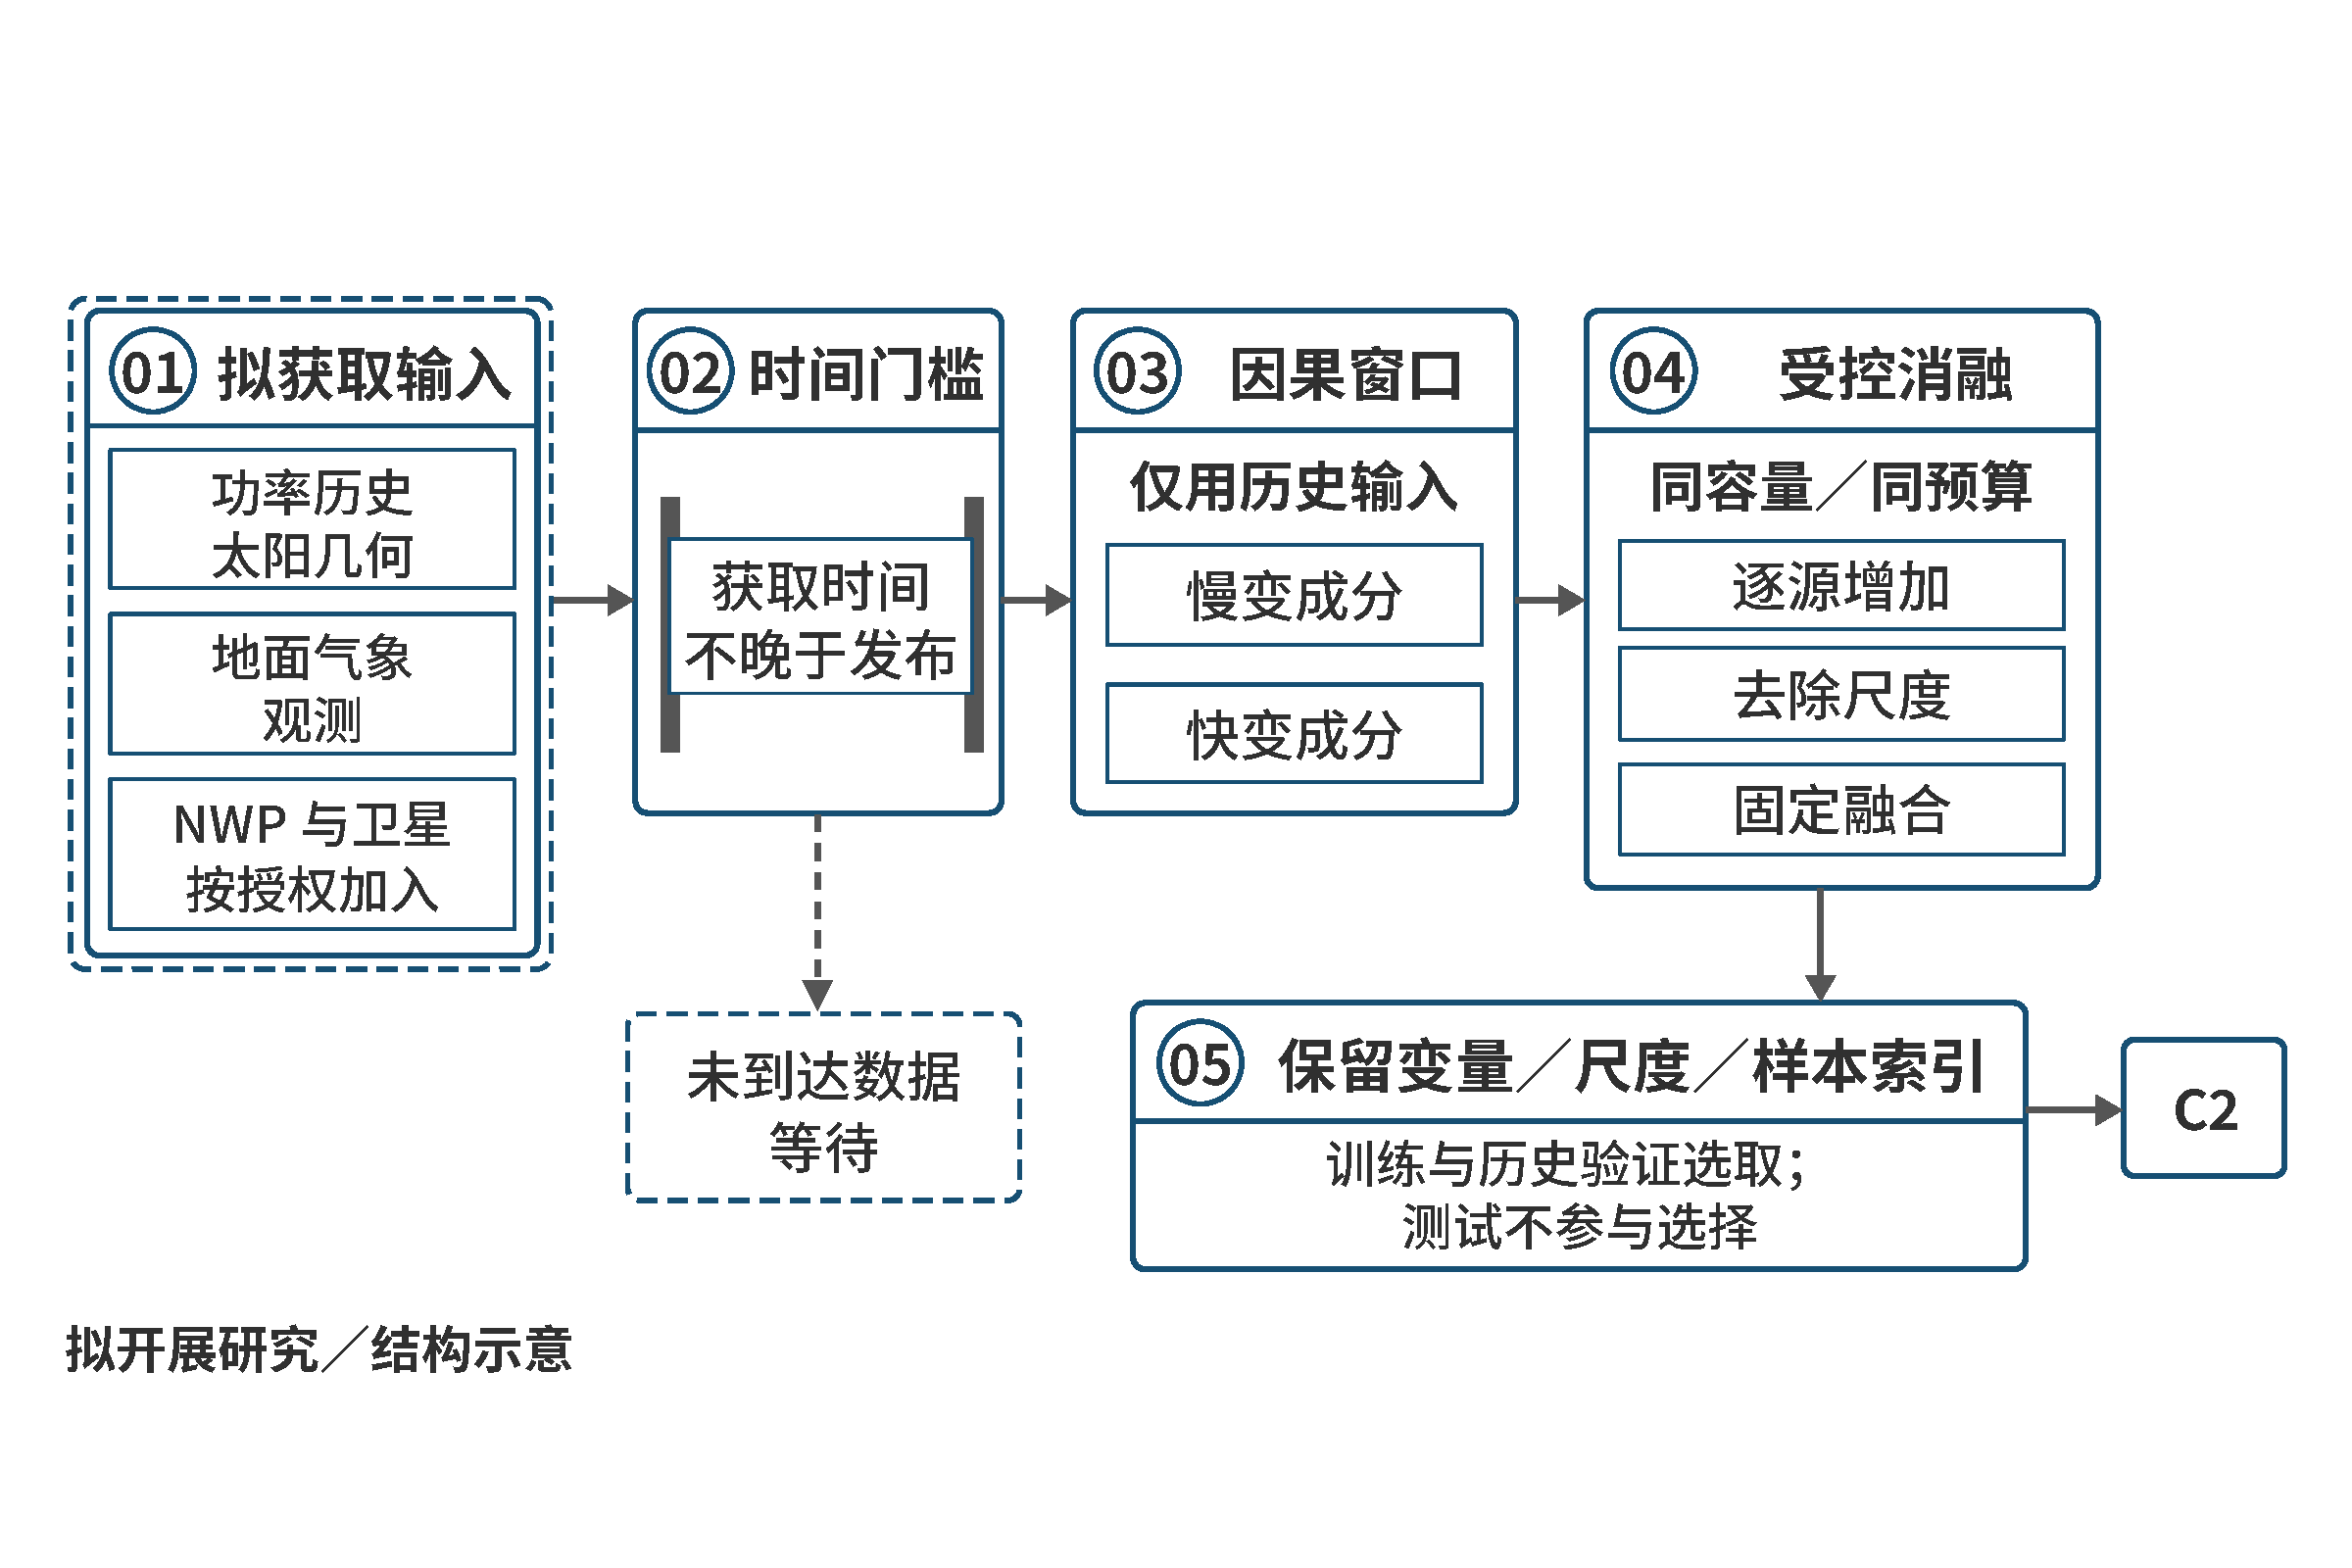
\includegraphics[width=0.94\linewidth]{figures/F03.pdf}
\caption{可用信息与跨尺度增益路线（数据按授权加入，变量选择不使用测试效果）}
\label{fig:xj-f03}
\end{figure}
% NSFC-ILLUSTRATED END F03

\subsubsection{对应研究内容二的路线}
输入经核验的样本和尺度特征，训练分位数模型，并以只含到达标签的滚动样本校准区间。输出原始单调分位数网格、单独校准的区间、覆盖诊断和完整历史误差轨迹，比较静态与滚动校准的覆盖及效率。原始分位数网格与误差秩模板一并传给内容三，校准区间用于并行可靠性诊断；不将两个覆盖层级的端点拼接成已校准的完整分布，不把区间覆盖结果当作事件可靠性的替代证据。
% NSFC-ILLUSTRATED BEGIN F04
如图~\ref{fig:xj-f04} 所示，分位数预测与延迟标签校准路线采用80\%与90\%两个覆盖层级。
\begin{figure}[htbp]
\centering
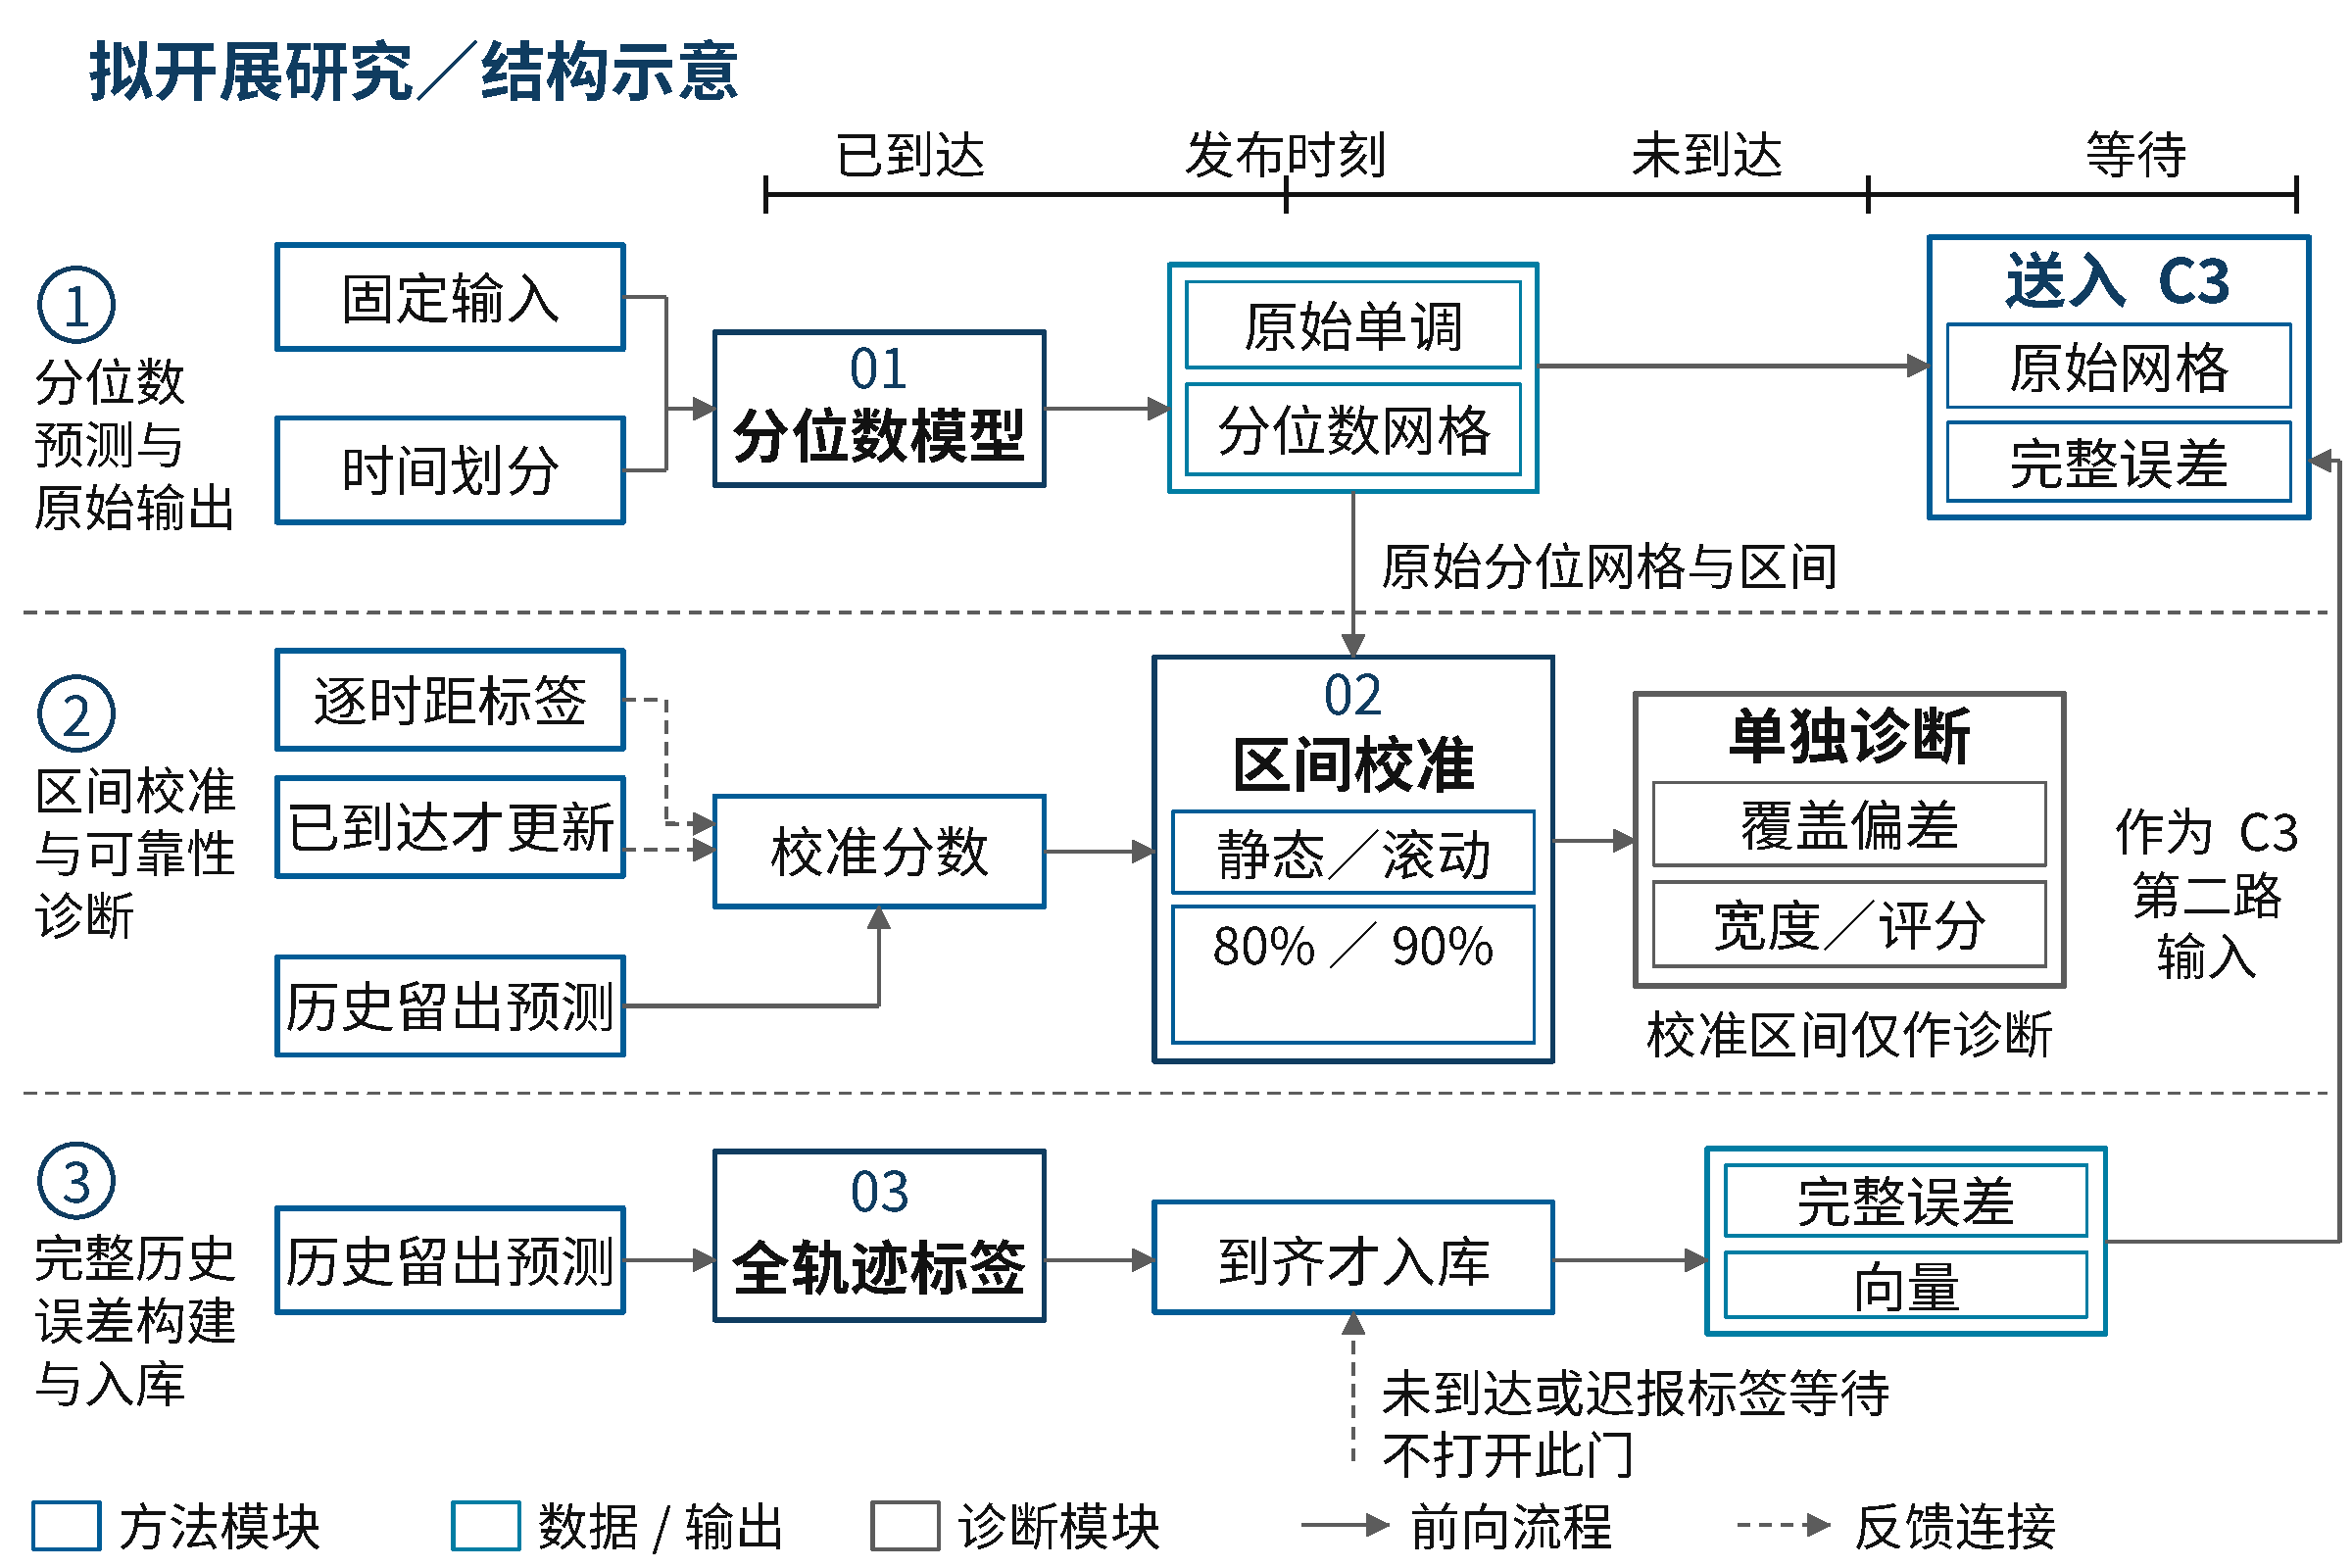
\includegraphics[width=0.94\linewidth]{figures/F04-confirmed.pdf}
\caption{分位数预测与延迟标签校准路线（80\%与90\%覆盖层级）}
\label{fig:xj-f04}
\end{figure}
% NSFC-ILLUSTRATED END F04

\subsubsection{对应研究内容三的路线}
输入内容二的边际预测与可用历史误差轨迹，构造同边际、不同时间依赖的轨迹并计算爬坡概率，与独立排序和直接增量方法对照。输出事件概率、可靠性分析与按事件聚合的告警记录，以概率评分和锁定告警规则下的实际效果验证，最后形成可回放的离线原型和适用条件说明。
% NSFC-ILLUSTRATED BEGIN F05
如图~\ref{fig:xj-f05} 所示，同边际依赖对照与爬坡评价路线（配对示意非实测，D0为主检验、D1为预设次检验）。
\begin{figure}[htbp]
\centering
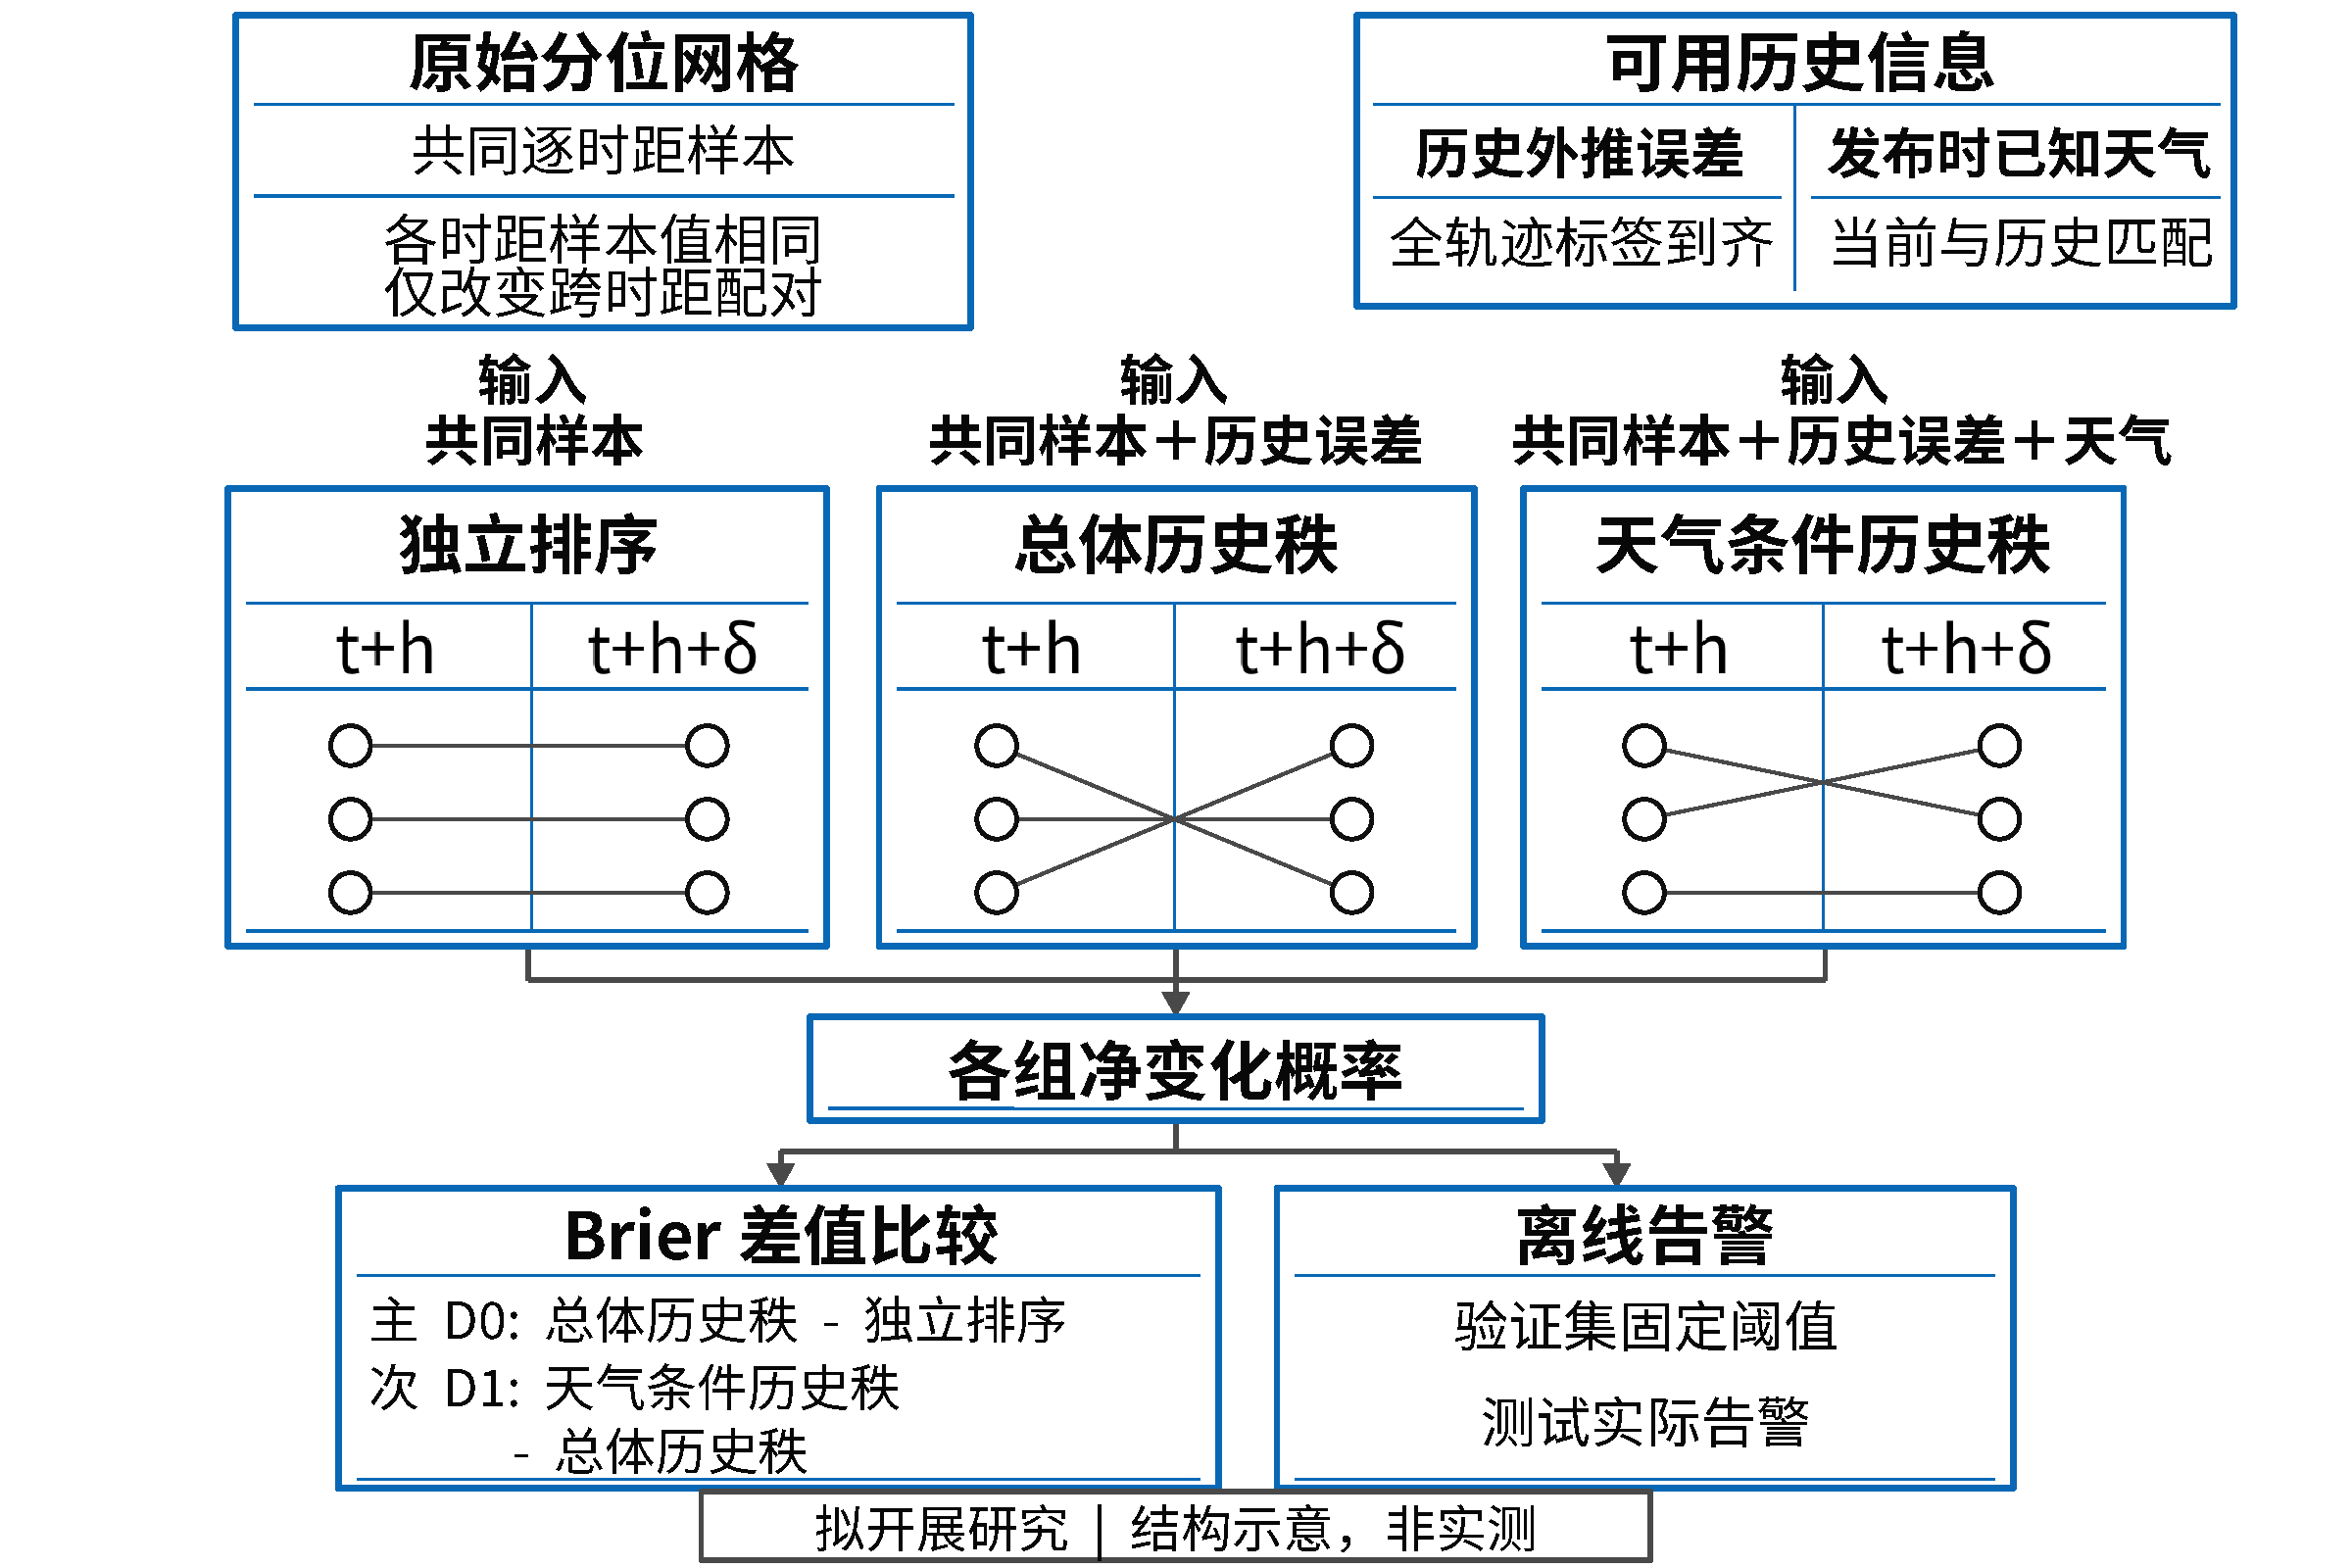
\includegraphics[width=0.94\linewidth]{figures/F05.pdf}
\caption{同边际依赖对照与爬坡评价路线（配对示意非实测，D0为主检验、D1为预设次检验）}
\label{fig:xj-f05}
\end{figure}
% NSFC-ILLUSTRATED END F05

\subsection{关键技术}
第一项关键技术是记录气象信息何时可用，并限定尺度变换只使用过去数据，使模型输入与实际发布情景一致。每项变量保留取得时间，分解和插补仅使用过去信息，理想输入对照与实际可用输入明确分开。

第二项关键技术是处理真实值到达延迟的概率校准。不同预测时距对应不同可更新样本，只有标签到达后才更新对应分数；小样本天气以诊断为主，防止分组过细造成虚假可靠性。

第三项关键技术是同边际的依赖结构对照。逐列相同、逐行配对不同的轨迹使时间依赖贡献可以被单独检验，再通过独立事件统计连接预警效果。三项技术均以能够复现实验和发现失效条件为要求，不以模块数量作为评价依据。

\subsection{可行性分析}
申请人已有光伏多尺度预测和长时序研究基础，可复用DWT-Former代码开展分位数建模、必要对照与后处理实验。现有GPU和软件工具支持单卡训练、多卡并行重复实验；由申请人负责研究设计与核查，\XJField{student-count}名新疆大学研究生分担数据、建模、校准、事件评价及原型任务，具体投入时间另行落实。首年建立数据和概率预测基线，次年完成校准与爬坡检验，实验规模与两年期限、3万元申请经费相匹配。

科学问题可以通过留出时段的覆盖偏差、区间评分和同边际轨迹差异检验；尺度、气象输入与校准的作用分别由消融实验辨别。主要实施条件是新疆实测数据及授权，业务NWP和第2场站用于扩展。仅有功率与历史观测时仍可开展短时主任务，但公开数据不能支撑新疆实测结论。数据与合作的落实状态在研究基础中列明，未满足条件时按以下节点调整任务。

\subsection{研究风险与应对措施}
\subsubsection{数据与进度风险}
新疆光伏实测数据或气象档案未按计划取得，将影响场景验证。拟在项目首季度核验授权、覆盖时段、时间戳和关键字段；若仍不能形成可用数据清单，则先在取得合法使用条件的公开数据上完成基线与评价流程，同时继续推进新疆数据获取。第一年度结束时若仍缺少足够的新疆数据，应明确缩小地域化验证范围，报告该目标未完成，不用公开数据或模拟功率替代新疆实测结论。

\subsubsection{概率预测技术风险}
天气分布变化和样本时间相关性可能使预测区间失准。若连续滚动评价窗口出现覆盖率偏离、区间显著变宽或爬坡概率校准恶化，拟比较滚动校准、按天气分组诊断与更简单的预测模型，分别报告不同情形下的结果。若复杂模型不能稳定优于基线，则保留较简洁模型及其适用范围，交付完整比较结果，不以训练集表现选择结论。

\subsubsection{罕见事件样本风险}
强爬坡或特定天气的独立事件过少，可能导致风险分级缺乏统计依据。若某一天气分层无法形成跨时间段重复评价，则回退总体历史模板，报告样本量与不确定性，不作该分层的定量优劣结论。非主要描述分组可按预定规则合并并明确标注；主事件定义、阈值和原始测试结果保持不变，避免为增加样本而调整判据。

\subsubsection{资源与合作风险}
业务数据授权、外部验证安排或共享算力的可用时间可能变化。拟优先采用已确认的计算资源，控制模型规模，以统一训练预算完成必要基线与消融。若合作验证不能落实，则保留可复现实验和离线原型，明确业务应用尚未验证；未经数据权利人许可，不公开原始场站数据。
